\clearpage{\pagestyle{empty}\cleardoublepage}

\chapter{Search for $T\bar{T}\to WbWb$ with pp collisions at \rts = 7~\tev}\label{app:wbx7tev}

Using 4.7\ifb\ of the data collected by the ATLAS experiment
in 2011 from pp collisions at a \cme\ of \rts = 7~\tev
the first quasi-model independent search for heavy vector-like
top quarks was performed~\cite{ATLAS:2012qe}. Originally designed for searches
of chiral fourth-generation top partners, this 
analysis is optimized for the $T\bar{T}\to WbWb$ 
decay channel.

\section{Analysis}

The analysis strategy as well as the event selection is
basically identical to what is described in Chapter~\ref{chap:wbx},
with minor differences mainly due to the different datasets
used (2011 data from pp collisions at \rts = 7~\tev~\cite{topCommonObjects2012}
versus 2012 data from pp collisions at \rts = 8~\tev~\cite{topCommonObjects2013}).
The \wbx\ search is, indeed, the upgrade of this analysis.
Small differences include also minor variations in the recontruction
of the boosted $W$ bosons (see also Figure~\ref{fig:7tevmwhad}): for the 7~\tev\ (8~\tev) analysis
the mass window is between 60\gev and 110 (120)\gev\ and \wii\ 
has $\pt(jj)>150 (200)\gev$. 


\begin{figure}[h!tb]\begin{center}
	\subfigure[]{\label{fig:7tevmwhadI}
          	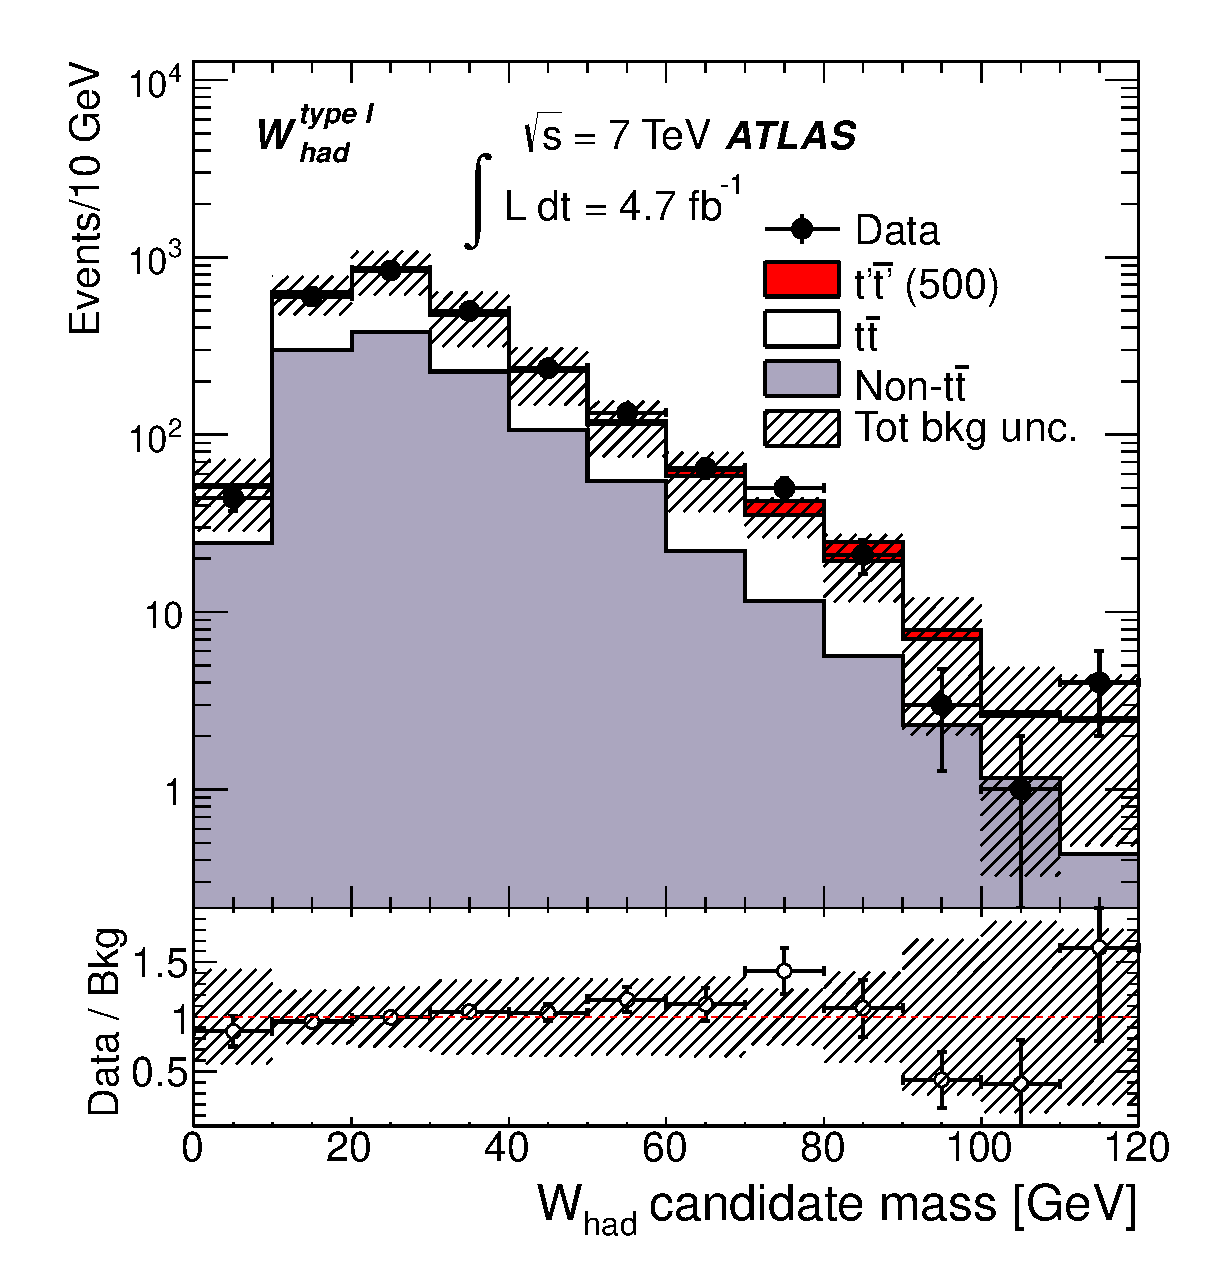
\includegraphics[width=0.47\textwidth]{appendices/figures/wbwb/fig_01a}}
	\subfigure[]{\label{fig:8tevmwhadI}
                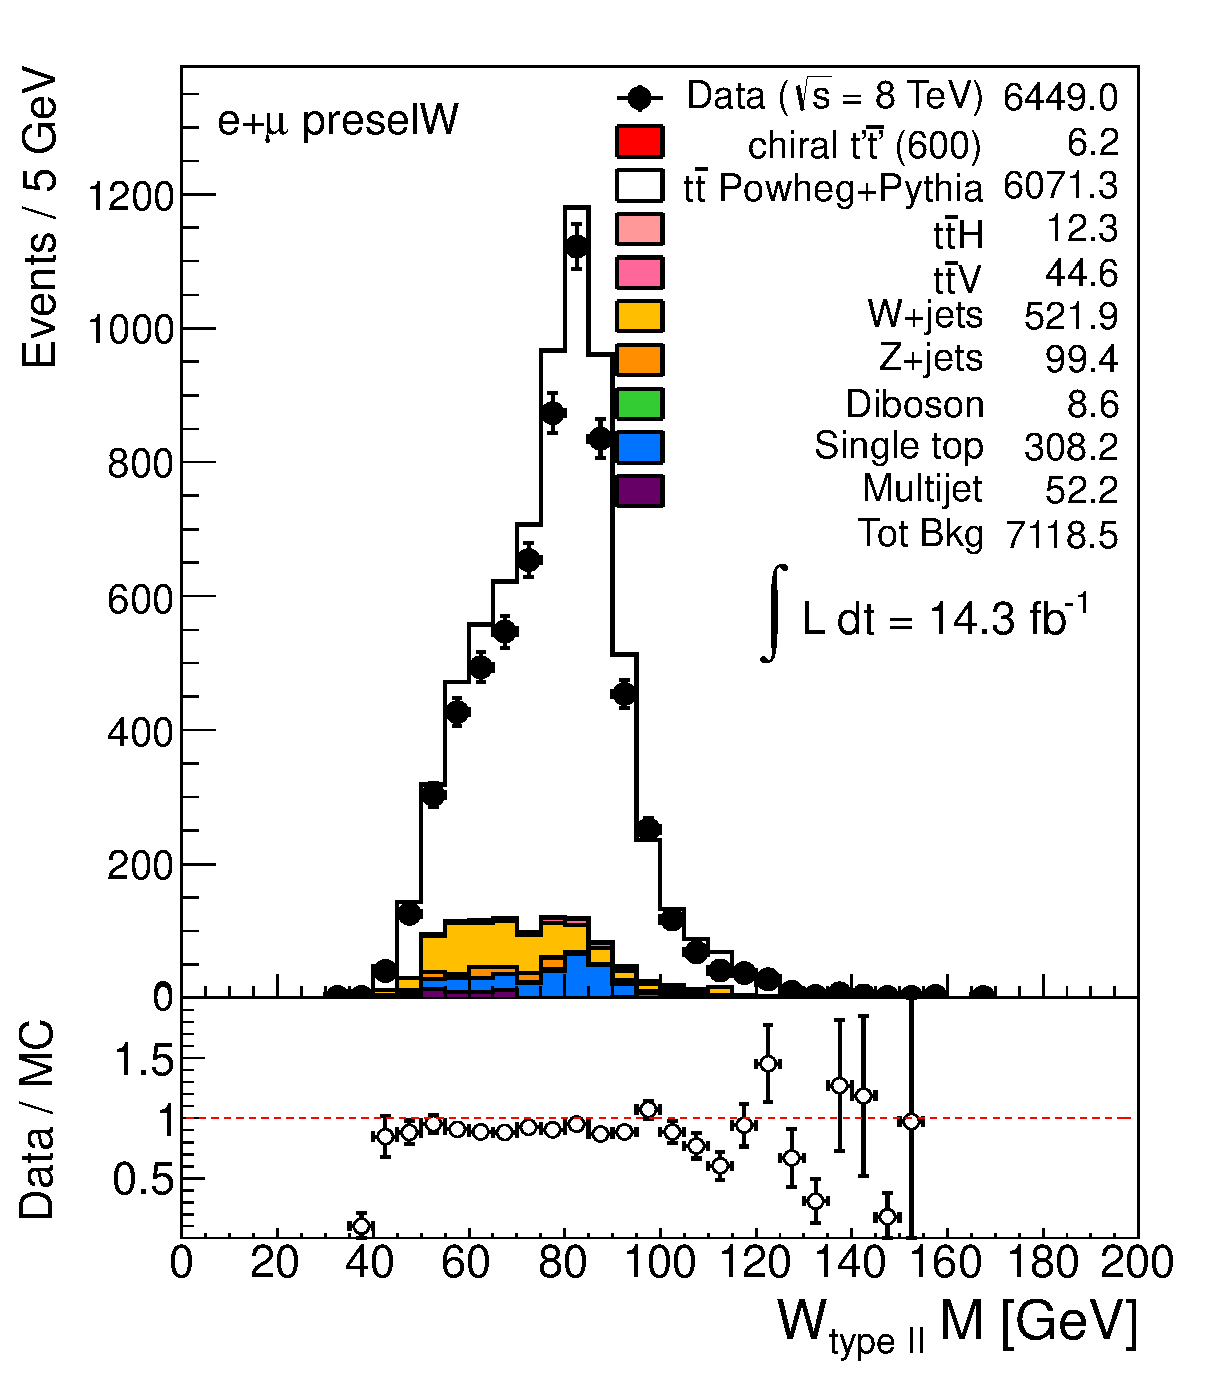
\includegraphics[width=0.45\textwidth]{wbx_analysis_14ifb/figures/confnoteplots/VLQAna_WbX_WpreselType2_M_ELEMUON_preselW_NOMINAL.eps}}\\
	\subfigure[]{\label{fig:7tevmwhadII}
          	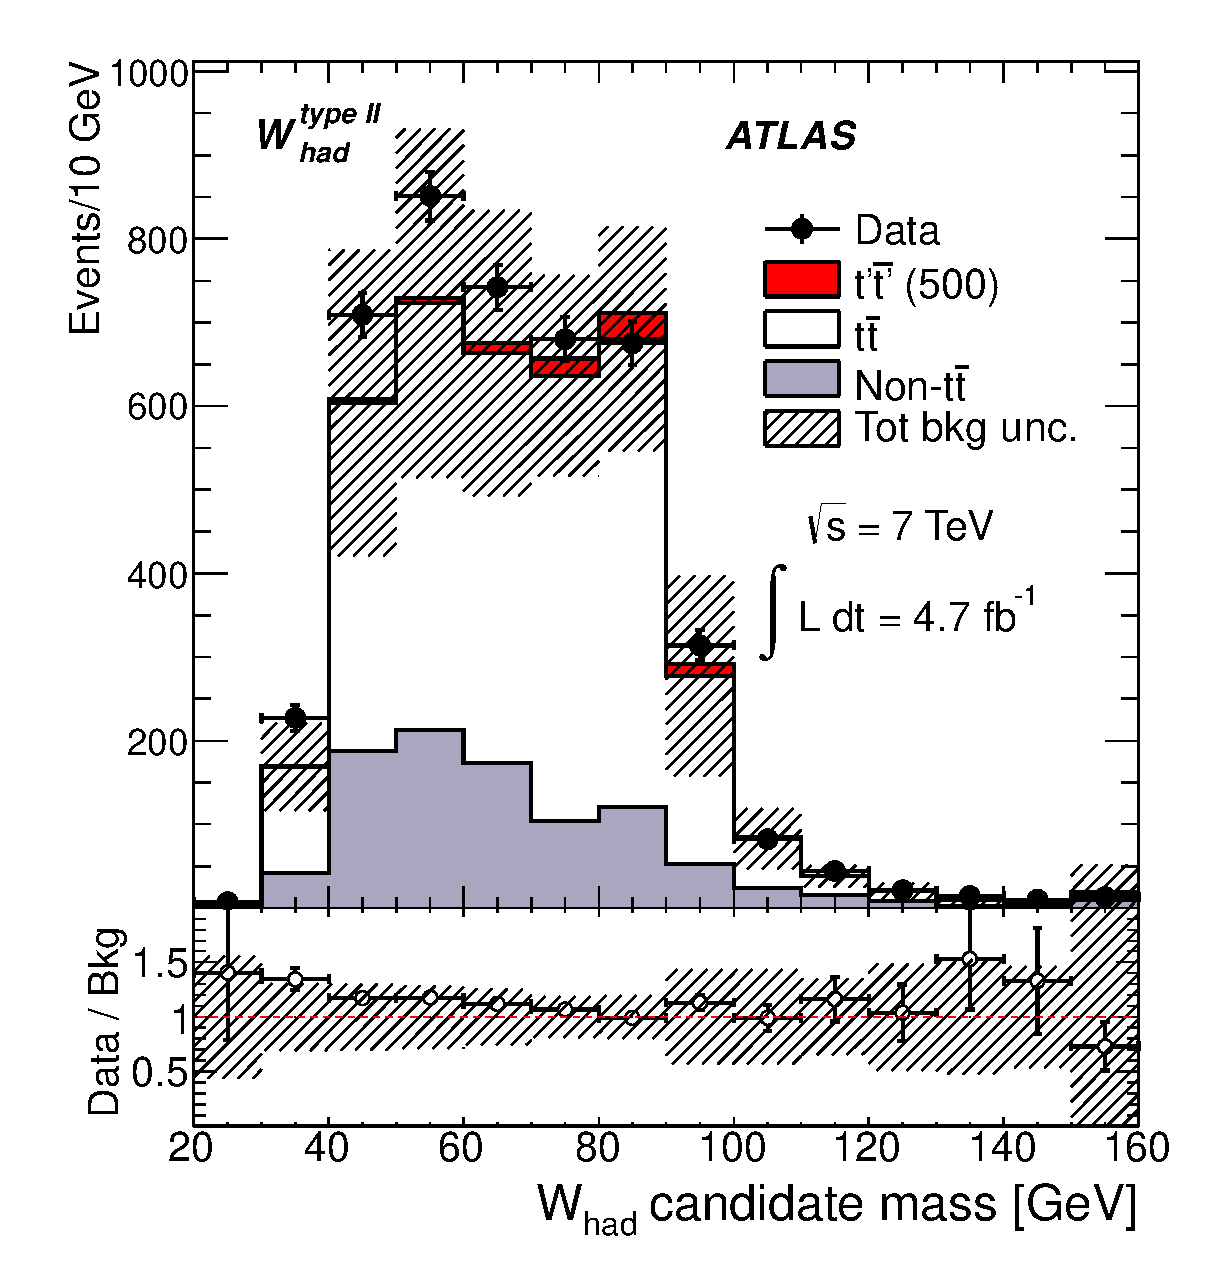
\includegraphics[width=0.47\textwidth]{appendices/figures/wbwb/fig_01b}}
	\subfigure[]{\label{fig:8tevmwhadII}
                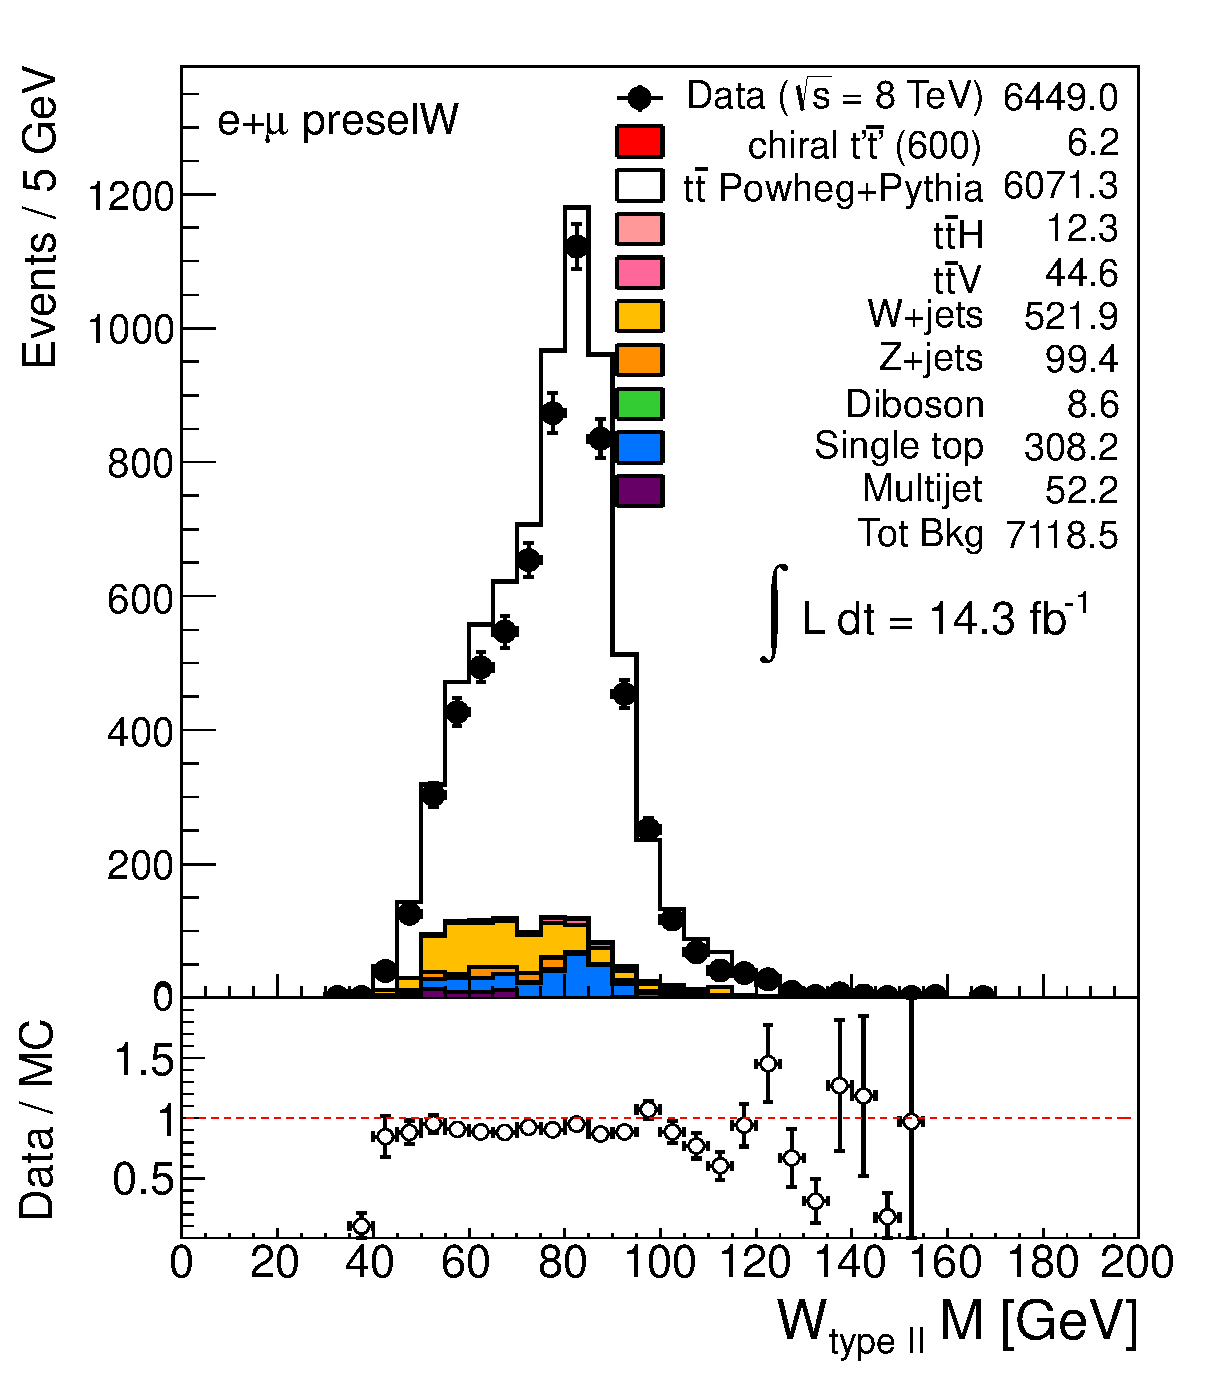
\includegraphics[width=0.45\textwidth]{wbx_analysis_14ifb/figures/confnoteplots/VLQAna_WbX_WpreselType2_M_ELEMUON_preselW_NOMINAL.eps}}
	\caption[bla]{Distribution of the reconstructed mass for 
        (a-b) \wi\ and (c-d) \wii\ candidates
        for the combined $e$+jets and $\mu$+jets channels after preselection,
        prior to apply the mass window cut, for the 7\tev\ (a-c) and 8\tev\ (b-d) analyses.
        %        The data (solid black points) are compared to the background 
        prediction from Standard Model (stacked histograms). 
        The total uncertainty on the background estimation (see 
        Section~\ref{sec:wbxSYS} for details) is shown as a black hashed band.
        The expected contribution from a chiral fourth-generation $T$ quark 
        with mass $m_{\T}=600\gev$, multiplied by a factor of 50, 
        is also shown (red dashed histogram).
        The lower panel shows the ratio of data to background prediction. 
        The overflow has been added to the last bin.

        \label{fig:7tevmwhad}}
\end{center}\end{figure}

Table~\ref{tab:wbx7tevselection} summarises and compares the event selections
of the two analyses. Figure~\ref{fig:78tevDRlnu} shows the
distributions for the $\Delta R(\ell,\nu)$ variable in the
two analyses, which easily justifies the different cut choice
in the new search. The discriminating variable used 
to build the binned log-likelihood ratio, in the same 
way as presented for the 8\tev\ search, is reconstructed
as described in Section~\ref{sec:wbxDISCR}. Figure~\ref{fig:7tevmreco}
show the distributions in the two search channels.
The results that were obtained are reported in the following section.

\begin{table}[htb]
\begin{center}
\begin{tabular}{p{3cm}cc}
\toprule
Selection & 7\tev & 8\tev \\
\midrule
%\multirow{10}{*}{Preselection} & \multicolumn{2}{c}{One electron or muon$^{(*)}$}  \\\cmidrule{2-3}
\ldelim\{{12}{12ex}[\hskip4ex Preselection] & \multicolumn{2}{c}{One electron or muon$^{(+)}$}  \\\cmidrule{2-3}
             & $\met >35(20)\gev$ for electron & $\met >20\gev$ \\
             &  (muon) channel & \\\cmidrule{2-3}
             & \multicolumn{2}{c}{$\met +m_{\rm T}>60\gev$} \\\cmidrule{2-3}
             & $\geq 3$ jets for \wi & \multirow{2}{*}{$\geq 4$ jets$^{(*)}$}\\
             & $\geq 4$ jets for \wii & \\\cmidrule{2-3}
             & \multicolumn{2}{c}{$\geq 1$ $b$-tagged jets$^{(**)}$} \\\cmidrule{2-3}
             & & orthogonality cut:\\
             & & reject events with $\geq 6$ jets \\
             & & and $\geq 3$ $b$-tagged jets \\
\midrule
%\end{tabular}
%\begin{tabular}{lll}
%\multirow{6}{*}{\loose\ selection} & \multicolumn{2}{c}{ Preselection } \\
\ldelim\{{6}{6ex}[\loose\ selection] & \multicolumn{2}{c}{ Preselection } \\
                  & \multicolumn{2}{c}{$\geq 1~W_{\rm had}$ candidates$^{(\rm x)}$} \\
                  & $\htfj>750\gev$ & $\htfj>800\gev$ \\
                  & \multicolumn{2}{c}{ $\pt(b_1) > 160\gev$}\\
                  & $\pt(b_2) >60\gev$ & $\pt(b_2) >80\gev$ \\
                  & $\Delta R(\ell,\nu)<1.4$ & $\Delta R(\ell,\nu)<1.2$ \\
\midrule
%\multirow{3}{*}{\tight\  selection} & \multicolumn{2}{c}{ \loose\ selection} \\
\ldelim\{{3}{3ex}[\tight\  selection] & \multicolumn{2}{c}{ \loose\ selection} \\
     	      & \multicolumn{2}{c}{ min$\Delta R(\ell,b)>1.4$}\\
              & \multicolumn{2}{c}{ min$\Delta R(W_{\rm had},b)>1.4$} \\
\bottomrule
\multicolumn{3}{c}{\footnotesize (+) Leptons have different $p_T$ thresholds and triggers. Both follow {\it topcommon} prescriptions.}\\
\multicolumn{3}{c}{\footnotesize (*) Jets in 7\tev\ (8\tev) analyses are calibrated at the EM+JES (LC+JES) scale.}\\
\multicolumn{3}{c}{\footnotesize (*) The $b$-tagging algorithm and working point for 7\tev\ and 8\tev analyses are the same: MV1, 70\%.}\\
\multicolumn{3}{c}{\footnotesize (x) The boosted $W$ reconstruction for 7\tev\ and 8\tev analyses is slightly different, see text.}\\
\bottomrule
\end{tabular}
\caption{Summary of event selection requirements for the 7\tev\ and 8\tev analyses.}
\label{tab:wbx7tevselection}
\end{center}
\end{table}

\begin{figure}[h!bt]\begin{center}
	\subfigure[]{\label{fig:7tevDRlnu}
                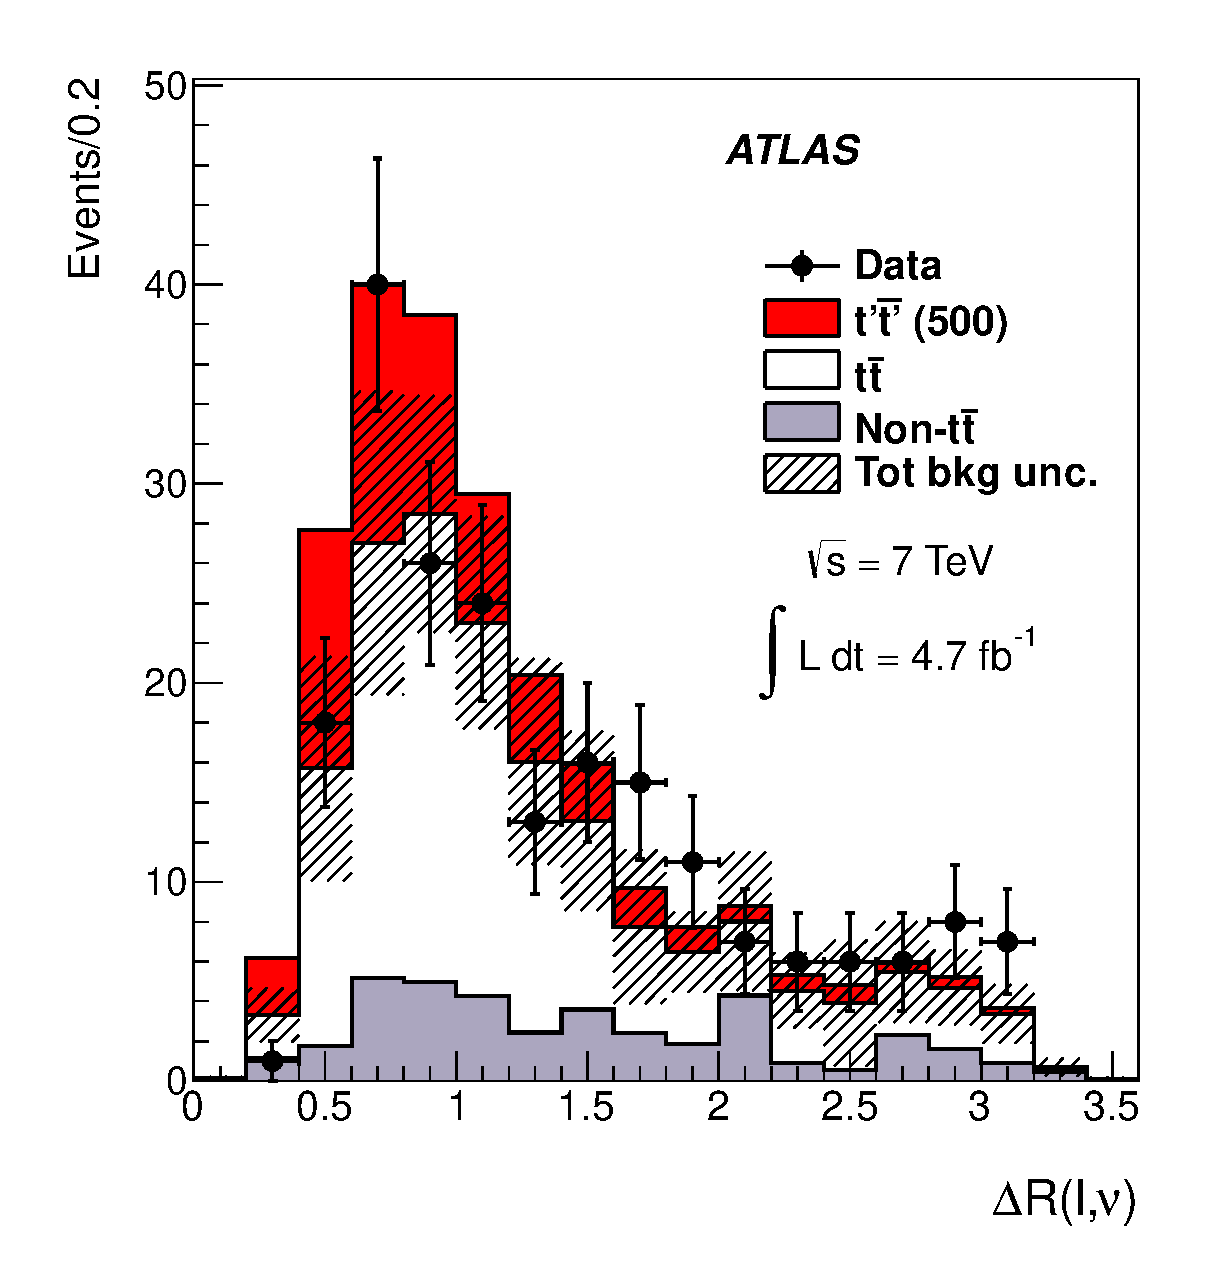
\includegraphics[width=0.47\textwidth]{appendices/figures/wbwb/figaux_08}}
	\subfigure[]{\label{fig:8tevDRlnu}
                \includegraphics[width=0.44\textwidth]{wbx_analysis_14ifb/figures/confnoteplots/VLQAna_WbX_DRLepMet_ELEMUON_cutflow1234_NOMINAL.eps}}
        \caption[bla]{Distribution of $\Delta R(\ell,\nu)$ in the (a) 7~\tev\ and
        (b) 8~\tev\ analysis after applying all previous selection requirements (see text for details),
        except for the requirements on $\Delta R(\ell,\nu)$ in the
        $e$+jets and $\mu$+jets channels.
        %        The data (solid black points) are compared to the background 
        prediction from Standard Model (stacked histograms). 
        The total uncertainty on the background estimation (see 
        Section~\ref{sec:wbxSYS} for details) is shown as a black hashed band.
        The expected contribution from a chiral fourth-generation $T$ quark 
        with mass $m_{\T}=600\gev$, multiplied by a factor of 50, 
        is also shown (red dashed histogram).
        The lower panel shows the ratio of data to background prediction. 
        The overflow has been added to the last bin.

        \label{fig:78tevDRlnu}}
\end{center}\end{figure}
\begin{figure}[h!tb]\begin{center}
	\subfigure[]{
  	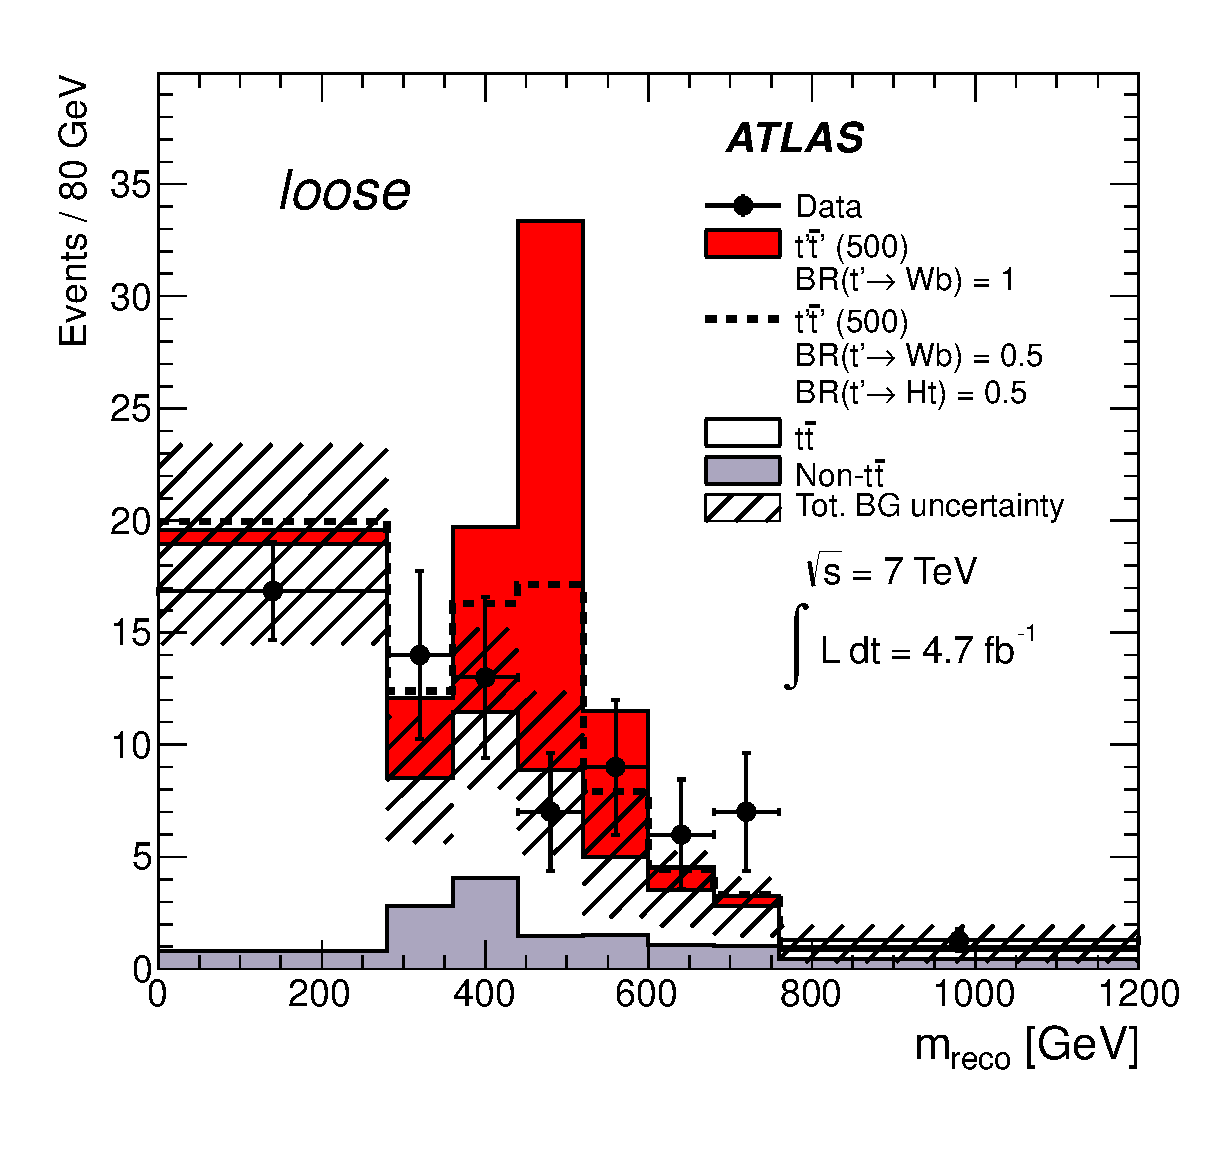
\includegraphics[width=0.45\textwidth]{appendices/figures/wbwb/fig_02a}}
	\subfigure[]{
  	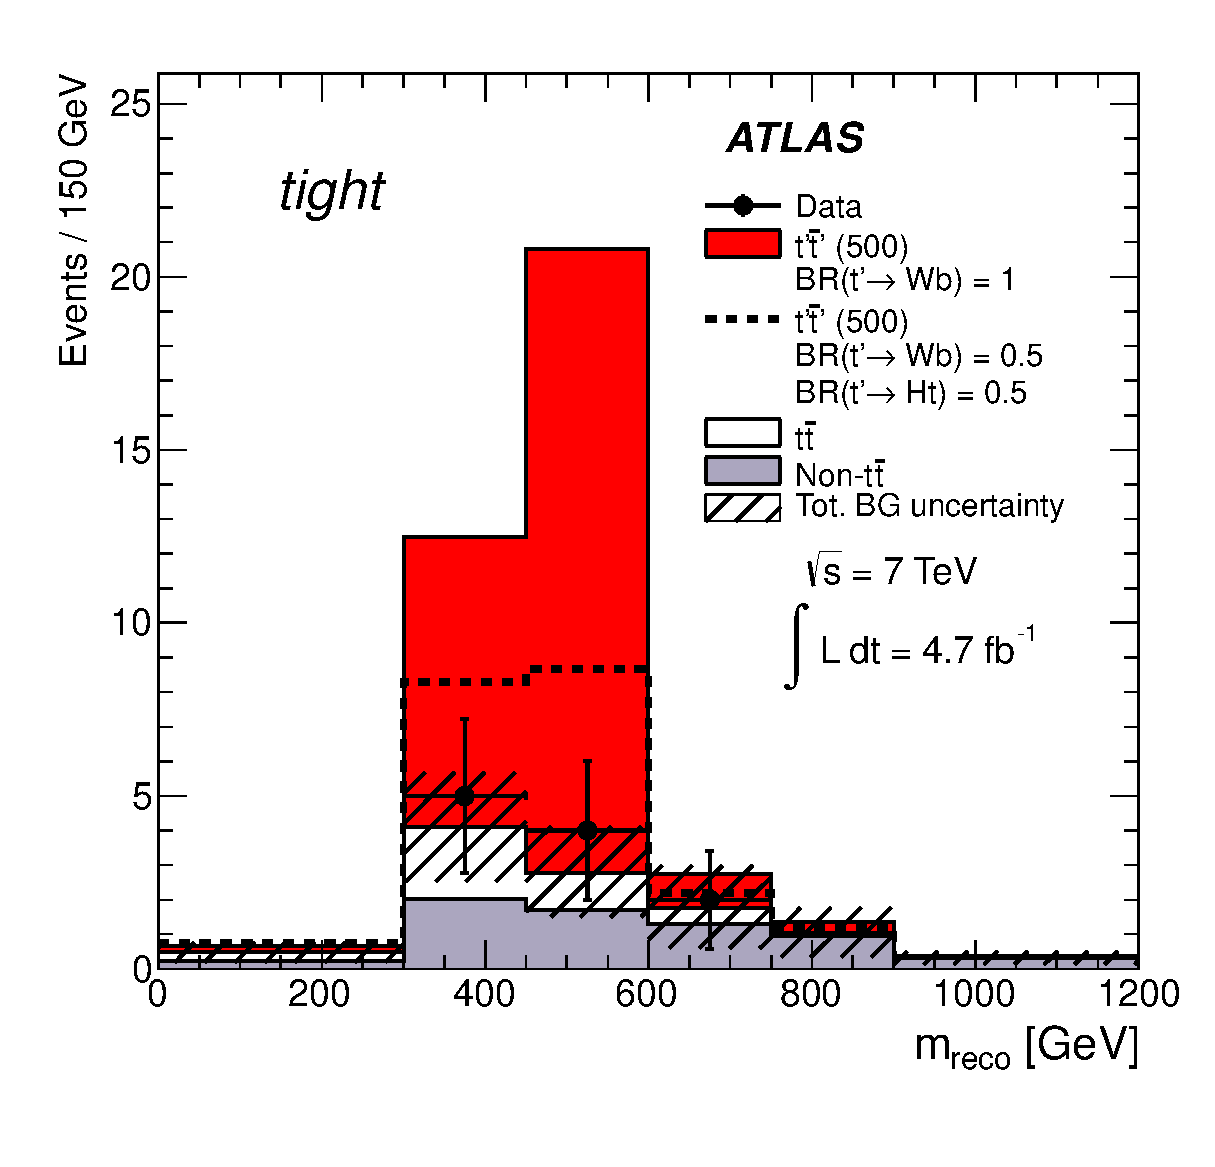
\includegraphics[width=0.45\textwidth]{appendices/figures/wbwb/fig_02b}}
	\caption{Reconstructed mass distribution in the (a) \loose\ and (b) \tight\ 
        channel for the 7\tev\ analysis.\label{fig:7tevmreco}}
\end{center}\end{figure}



\section{Results}

The Branching Ratio plane was originally proposed in
this analysis, with the aim of generalizing the
search for a fourth generation chiral top partner $t'$.
The strategy for building it is, therefore, the same as presented in
Section~\ref{sec:strategy}.
The obtained
exclusion for vector-like $T$ for different models is
shown in Figure~\ref{fig:7tevwbwb}.
The 95\% CL limits obtained for a
fourth generation chiral top partner
as a function of its mass are shown in Figure~\ref{fig:7tevCL}.


\begin{figure}[h!tb]\begin{center}
	\subfigure{
  	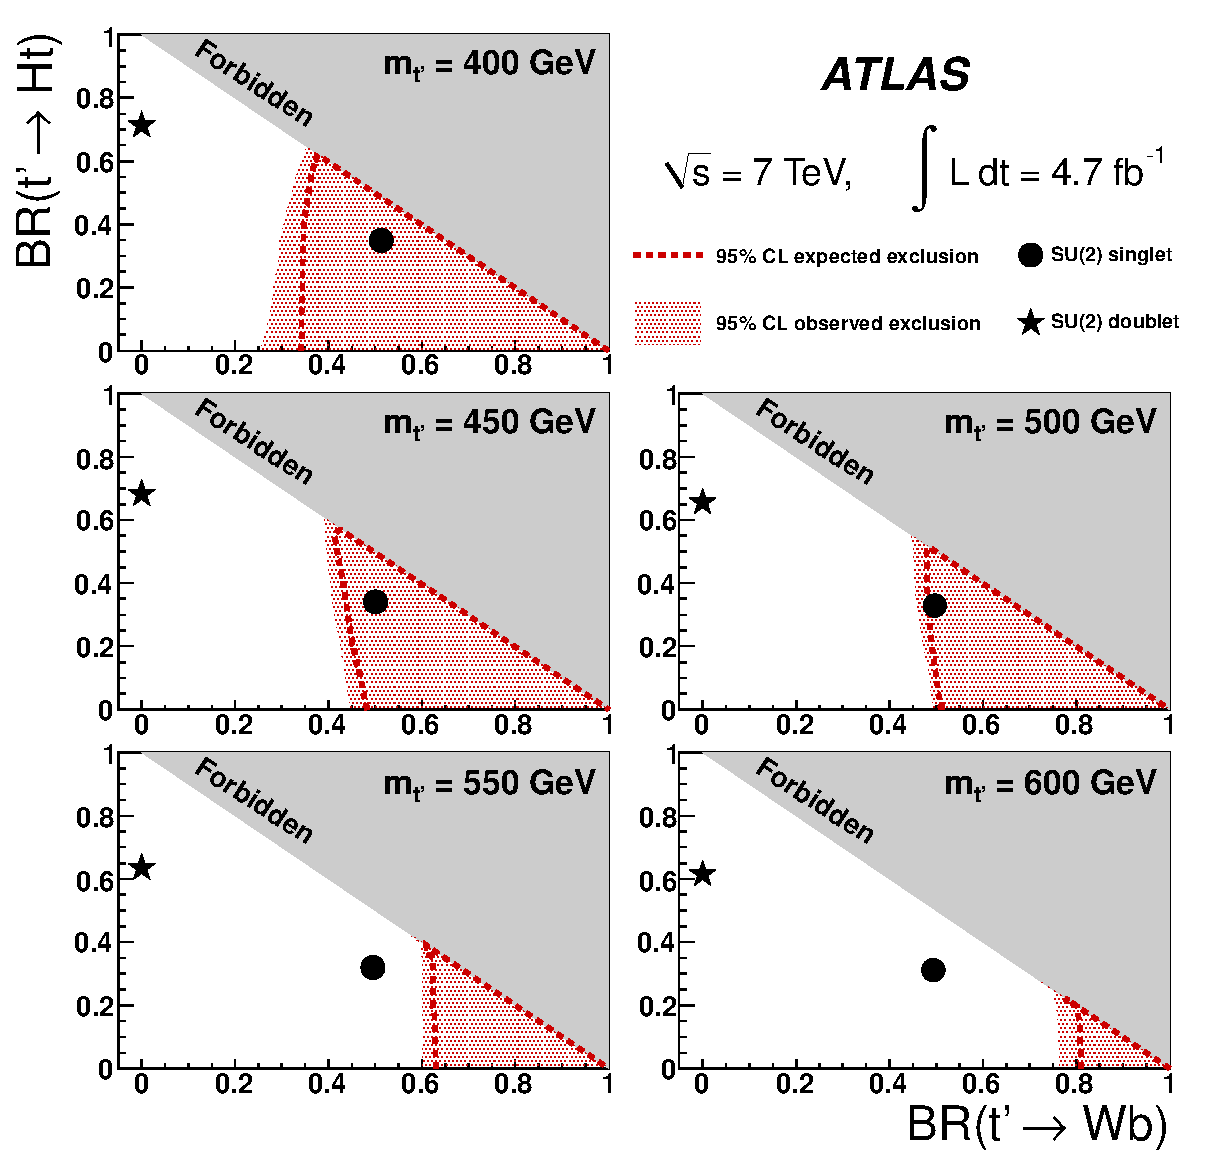
\includegraphics[width=0.85\textwidth]{appendices/figures/wbwb/fig_04}}
	\caption{Observed (red filled area) and expected (red dashed line) 95\% CL exclusion on the plane of BR($T\to Wb$) vs BR($T\to Ht$), 
for different values of the vector-like $T$ quark mass~\cite{ATLAS:2012qe}.  The
grey area corresponds to the unphysical region where the sum of branching ratios exceeds unity. 
The weak-isospin singlet and doublet points are shown as plain circle and star symbols, respectively.\label{fig:7tevwbwb}}
\end{center}\end{figure}
\begin{figure}[h!tb]\begin{center}
	\subfigure{
  	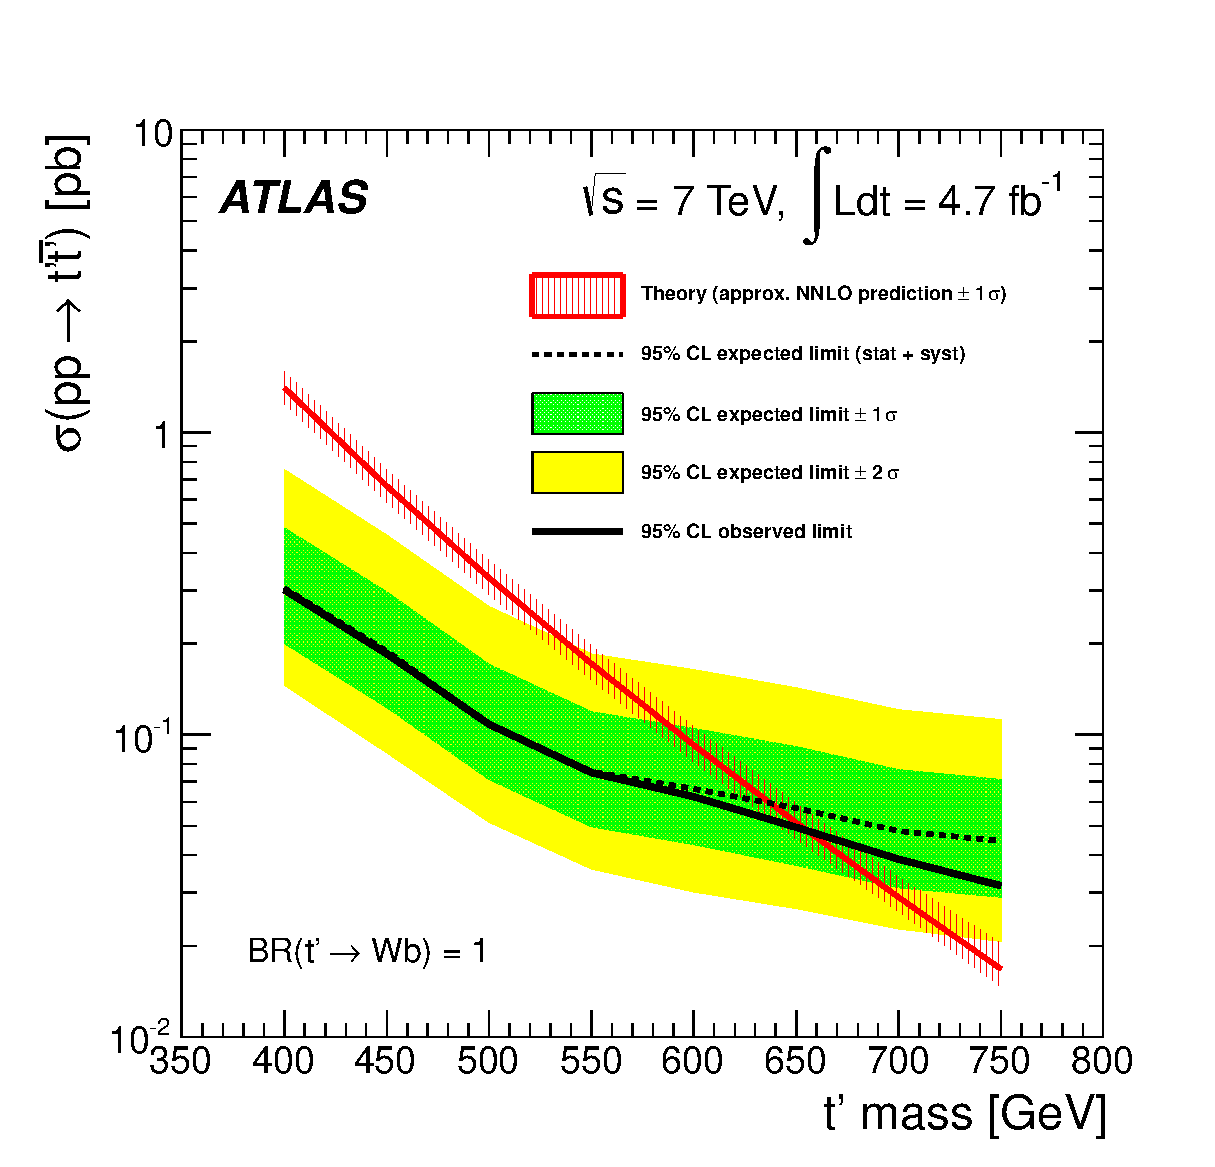
\includegraphics[width=0.7\textwidth]{appendices/figures/wbwb/fig_03}}
	\caption{Observed (solid line) and expected (dashed line) 95\% CL upper limits on the \TTbar\ 
        cross-section as a function of the \T\ quark mass. The surrounding shaded bands correspond 
        to the $\pm$1 and $\pm$2 standard deviations around the expected limit. 
        The thin red line and band show the theoretical prediction and its $\pm$1 standard deviation uncertainty. \label{fig:7tevCL}}
\end{center}\end{figure}
